
\chapter{مقدمه ای بر توصیف رسمی برنامه ها و سیستم ها}\label{chapter1}
\paragraphfootnotes
امروزه به همراه هر نرم افزار و یا سیستمی، مجموعه وسیعی از مستندات نیز ارائه می شود. این مستندات شامل : راهنمای کابر، کتاب راهنمای مرجع 
\LTRfootnote{reference manuals}
، سیستم های راهنمای آنلاین، آموختارهای تعاملی
\LTRfootnote{interactive tutorials}
 و مستندات طراحی است. با این حال، رفتار نرم افزار، همچنان برای کابران و طراحان، غافل گیر کننده می باشد. گاها مولفه های برنامه به درستی عمل نکرده و سیستم در مواجهه با نیازمندی های کاربر، با شکست مواجه می شود.
 
 در علوم کامپیوتر، توصیفات رسمی، تکنیک‌های مبتنی بر ریاضیات هستند که هدف آنها کمک به پیاده‌سازی سیستم‌ها و نرم‌افزارها است. توصیف ها برای شرح چگونگی عملکرد یک سیستم، تحلیل رفتار سیستم و بررسی و تایید مشخصات کلیدی آن بکار برده می شوند. این توصیفات رسمی هستند به این معنا که دارای یک نحو هستند، از لحاظ معنایی در یک دامنه قرار می گیرد و می توان از آنها برای درک و دریافت اطلاعات مفید استفاده کرد.

تحلیل نیازمندی ها و توصیف آنها، مبتنی بر ارتباط بین کارفرما، کاربران و تحلیل گران و توسعه دهندگان سیستم است. روش های معمول تحلیل و طراحی سیستم های نرم افزاری، به میزان زیادی، متکی بر زبان های طبیعی و نمادهای گرافیکی است. به این ترتیب ممکن است در توصیف یک سیستم نرم افزاری مشکلات زیر رخ دهند:
\\
1. تناقض: بیان های متفاوت از موضوعی واحد در قسمت های مختلف مستند نیازمندی ها.
مثلا در یک قسمت پایش دما در تمامی حالات خواسته شده است و در بخشی دیگر، در محدوده ای خاص
\\
2.  ابهام: امکان وجود برداشت های مختلف از یک عبارت خاص.
(مثلا در جایی که در مستند نیازمندی ها پراگراف زیر نوشته شده است، مشخص نیست که جمله آخر درخصوص گذرواژه است یا شناسه کابر.
\\
"شناسایی کاربر بوسیله نام کاربری و گذرواژه صورت می گیرد. که باید ترکیبی از حروف و ارقام باشد.
\\
3. غیردقیق بودن: غیردقیق بودن به این معناست که در بیان نیازمندی ها، عبارات کلی گفته شود.
(به عنوان مثال در عبارت " فاصل کاربری، باید کاربرپسند باشد" دقیقا مشخص نشده که منظور از کاربر پسند بودن چیست و به بیان این نیاز، بصورت کلی بسنده کرده است.)
\\
4. کامل نبودن
\\

روش های رسمی از منطق و ریاضیات ساده برای بیان نیازمندی های یک سیستم یا نرم افزار استفاده می کنند. همچنین در توصیف های رسمی از فرمول ها، نمادها و قواعد، استفاده می شود. با استفاده از توصیف رسمی، درک بهتر از سیستم در حین تحلیل سیستم فراهم می شود در حالیکه در سیستم های فاقد توصیف رسمی، این درک و دریافت، بعد از ساخت و با تست سیستم، فراهم می شود. در واقع یکی از اهداف اصلی توصیف های رسمی، آشکارسازی خطا در زمان تحلیل و نه در زمان تست و بعد از ساخت و تجربه کاربر است. در این روش ها، تحلیل بصورت خودکار و با استفاده از ماشین، انجام می شود.از جمله ایرادات توصیف های رسمی می توان به موارد زیر اشاره کرد:
\\
1. در کنترل پروژه کاربرد ندارند.
\\
2. مستندات آن برای مشتری، مفید و قابل درک نیست.
\\
3. برای پروژه بصورت هزینه سربار است.
\\
4. نباید آن را به عنوان جایگزینی برای تست ها درنظر گرفت

\section{اولین مثال از توصیف رسمی یک برنامه}\index{example of specification}
به تصویر \ref{pythoncode} که یک برنامه ساده در زبان پایتون است توجه کنید. این برنامه چه کاری انجام می دهد؟

\begin{figure}[!t]
\centering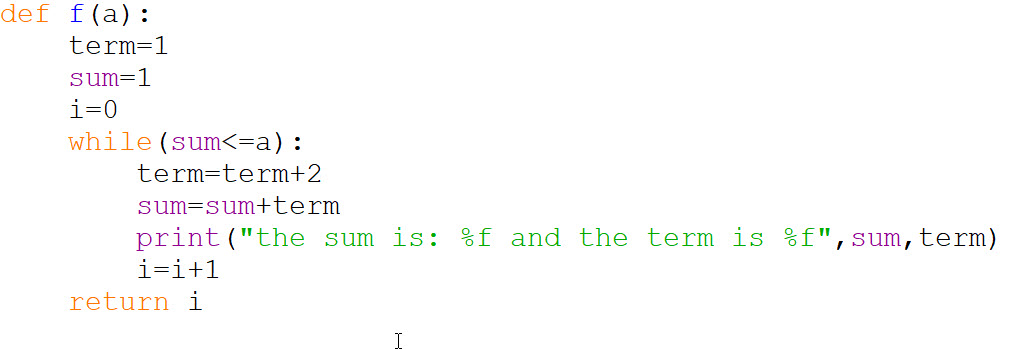
\includegraphics[width=\textwidth]{pythoncode}
\caption{
تعریف تابع در پایتون
}\label{pythoncode}
\end{figure}

با توجه به تعریف تابع 
$f(4)=2$
، اما اگر 
$a=10$
و یا
 $a=-10$
 باشد، آنگا تابع چه مقداری را برمی گرداند.
 \\
 برای درک بهتر کد پایتون شکل \ref{pythoncode} می توان نام تابع را به
  $ iroot $
تغییر داد و یک خط توضیحات به آن اضافه کرد (شکل \ref{pythoncodewithcomment}).

\begin{figure}[!t]
\centering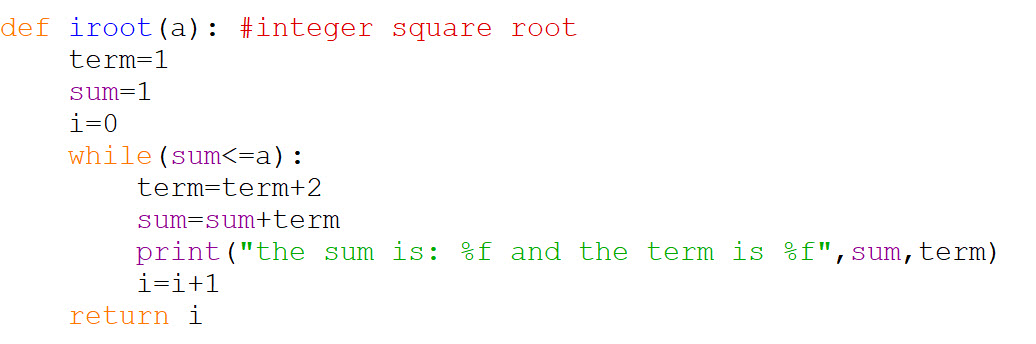
\includegraphics[width=\textwidth]{pythoncodewithcomment}
\caption{
تعریف تابع در پایتون به همراه توضیحات بیشتر
}\label{pythoncodewithcomment}
\end{figure}


 در اینجا متوجه می شویم که در توضیح این تابع، به چیزی بیشتر از کد نیاز داریم. کد، نحوه محاسبه خروجی را نشان می دهد در حالیکه "توصیف" نتیجه محاسبه را دربردارد. توصیف کد شکل
 \ref{pythoncode}
به زبان توصیف رسمی Z، به شکل \ref{iroot} خواهد بود.

\begin{figure}
\centering
\begin{schema}{iroot}
iroot :   \mathbb{N} \longrightarrow \mathbb{N}
\where
\forall a: \mathbb{N}\\
iroot(a) \ast iroot(a) \leq a < ( iroot ( a ) +1 ) \ast ( iroot ( a ) +1 )\\
\end{schema}
\caption{توصیف کد پایتون بوسیله زبان توصیف رسمی Z}
\label{iroot}
\end{figure} 
از توصیف رسمی، نمی توان به کد رسید. در توصیف برنامه، مشخص می شود که برنامه چه کاری انجام خواهد داد و در واقع به پرسش 
$ what $
پاسخ داده خواهد شد. اما کد پایتون برنامه مشخص می کند که چگونه این کار انجام می شود و پاسخ به پرسش
$ How $
را دربردارد. این دو تکمیل کننده یکدیگرند و در طراحی یک سیستم و یا یک نرم افزار، به هر دو نیاز داریم.
از مثال مطرح شده می توان به این نتیجه رسید که زبان های توصیف رسمی، زبان برنامه نویسی نیستند به این معنا که برای آنها کامپایلری که بتواند کد قابل اجرا تولید کند، وجود ندارد.
